\section{Results}


\begin{figure*}[ht]
    From the records of eleven geophones, the following plot shows all numerical timeseries recorded by SmartSolo devices, 
    excluding only timeseries for relating to device memory
    \centering
    \includegraphics[width=\textwidth]{reportImgs/12geoPhones.png}
    \caption{Numerical Data Plots for 11 Geophones}    
\end{figure*}

A few things stand out in this image. The orientation measures strongly correlate with temperature. This is undesirable, but can be fixed with a detrending. 
The high gain device used more power. The positions of some of the geophones were swapped when they were redeployed on the 3rd. 
Latitude and Longitude averages were then exported to google earth to generate the following plot:
\begin{figure*}[h]    
    \centering
    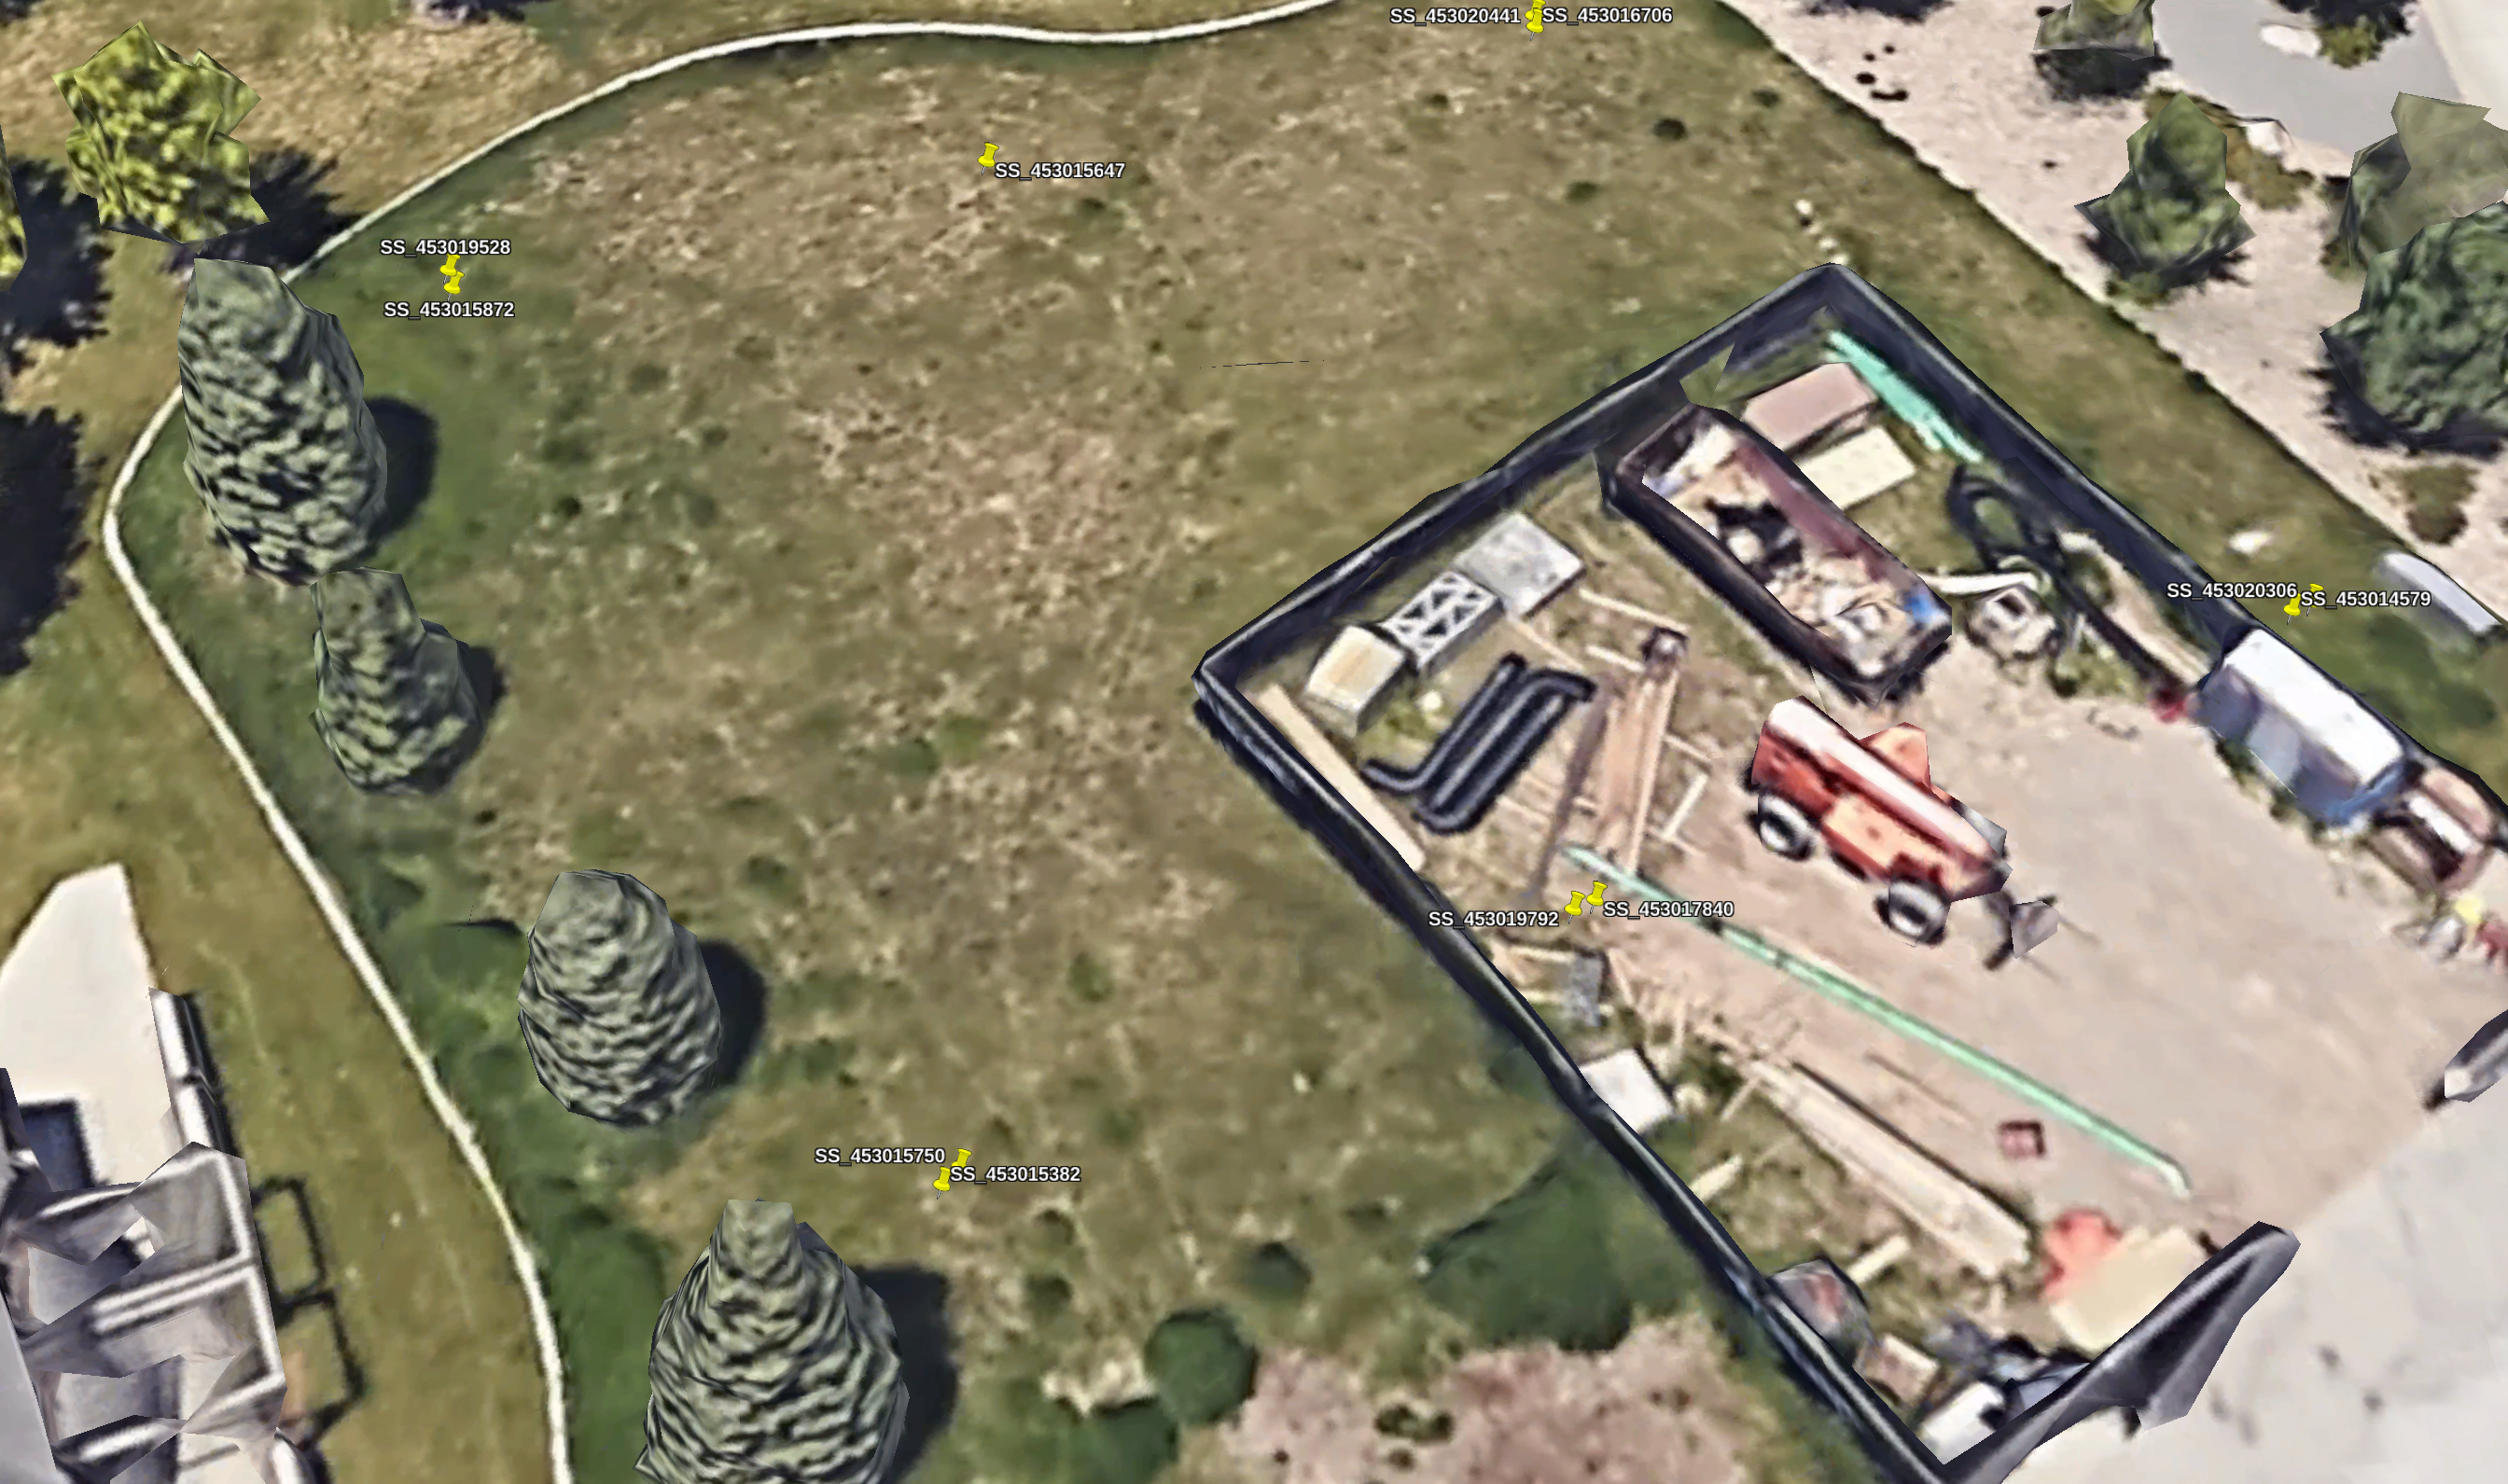
\includegraphics[width=\textwidth]{reportImgs/earthPlot.png}
    \caption{positions for 11 Geophone deployment}    
\end{figure*}

Between the image and current state of the field position error of the deployment is undifferentiable. From the standard deviation of the latitude and longitude time series, the precision is given to about half a meter. 
However, it is observed that the magnitude and direction of error is nearly the same between geophones, and therefore the measured distance between them is even much more accurate than that. The precision 
of the small distance between the closely deployed pairs of geophones is clearly visible in the google earth figure. 




\begin{figure*}[h]    
    \centering
    \includegraphics[width=\textwidth]{reportImgs/high_gainPlot.png}
    \caption{positions for 11 Geophone deployment}    
    \label{wf}
\end{figure*}

A sample waveform collection is plotted in \ref{wf}. It appears there may have been a seismic event recorded at about 9:00 UTC. However, by generating a spectrogram with obspy, a much better understanding of of the signal can be read.

\begin{figure}[h]
    \centering
    \includegraphics[width = \textwidth]{reportImgs/spectrogram1.png}
    \caption{The spectrogram of the waveform in \ref{wf}}    
    \label{spect1}
\end{figure}

With most of the sample rates set to 1000 hz, the amount of data collected from  eleven three channel geophones  was massive, 134.5GB. Such large datasets make operations such as channel orientation adjustments incredibly slow and cumbersome. 
However, a review of data  shows the geophones were able to recieve virtually no signal above 100 hz

\begin{figure}[h]
    \centering
    \includegraphics[width = \textwidth]{reportImgs/frResponse.png}
    \caption{The spectrogram of the waveform in \ref{wf}}    
    \label{fr}
\end{figure}
